% created on 30/03/2020
% @author : ebazan
\chapter*{Introduction}
\addcontentsline{toc}{chapter}{Introduction}
In this thesis we present the study of low-level primitives of an image such as contours, color, texture and texture color in search of generating vision algorithms useful for autonomous navigation of Unmanned Aerial Vehicles (UAVs). Since they allow to characterize objects in images under various conditions, these primitives have widely been used in image segmentation and modeling tasks. To go further, we take interest in the study of these primitives in combination with some concepts of human visual perception in order to achieve the understanding of scenes. In addition, we favor traditional Computer Vision (CV) methods that allow us to obtain image features that have a physical sense and that can be used later in completely unsupervised algorithms.

\section*{Background and Motivation (Relationship between drones and computer vision)}

The advancement of computer vision techniques has favored its use in a wide range of applications. The development has been outstanding in already traditional application areas such as multimedia or medicine. However, new areas of application continue to emerge such as augmented reality, automated driving, robotics, the Internet of Things (IoT) and the Industry 4.0, human-computer interaction and vision for the blind. 

Regardless of the application, computer vision systems must perform a number of tasks to achieve their goal. Generally, these tasks include methods for acquiring, processing, analyzing, and understanding digital images; extracting real-world data to produce symbolic information, for example, in the form of decisions. Depending on the context, understanding images can mean transforming visual images (the sensor input) into descriptions of the world that can interact with other processes and provoke appropriate actions. This compression can be seen as the crumbling of the symbolic information in the image using geometric, physical, statistical or theory of learning models.

More particularly, the tasks of computer vision can be grouped into four more or less well-defined processing problems.

\begin{enumerate}[label=\roman*]
	\item Recognition, a classic problem of computer vision which is responsible for determining whether an image contains any object, characteristic or exercise. Some variants of this problem are the classification, identification and detection of objects from which many specialized tasks emerge, for example, content-based image search, pose estimation, optical character recognition, reading of 2D codes, facial recognition, shape recognition, among others.
	\item Motion analysis, in which a sequence of images is processed to produce an estimate of the speed of one or more points of interest within a 3D image or scene. Some examples of this task are egomotion, object tracking, and optical flow.
	\item Scene reconstruction, which is a task related to the computation of a 3D model from one or more images of a scene.
	\item Image restoration, whose objective is to remove those imperfections of an image generated by disturbances such as sensor noise or motion blur. Generally this task done in the pre-processing stage of the image, before passing it to a more complex algorithm. An example in which this task is applied is inpainting.
\end{enumerate}

While computer vision has outstripped the capabilities of human vision, computers have not completely replaced human personnel. For example, in the case of industrial vision systems tasks, say inspecting bottles or circuit boards on a production line, CV algorithms surpasses humans. However, in areas such as medical imaging, computer vision systems are only responsible for supplementing certain routine diagnoses that require a lot of time and experience from human doctors. This is largely related to the complexity of the task and the conditions under which the application is carried out. In the case of machine vision systems, working conditions are generally controlled, while in areas such as medicine, each patient image is different despite the fact that the acquisition system is the same. We can see a similar effect in other areas such as robotics but in particular with unmanned aircraft.

Unmanned aerial vehicles (UAVs) or drones are these flying engines that are increasingly present in our lives. We can found them in various sectors, such as the military, commercial or civil, where they are able to carry out specific tasks quite efficiently. However, in most cases the development of such applications requires an expert pilot to control the aircraft. Commonly, the UAV  control is achieved with the use of conventional sensors, such as inertial sensors (IMUs) for orientation, and GPS for position. The combination of information from these sensors in a flight computer allow the drones to remain stable in the air. The drawback with the IMU is that suffers from bias error propagation due to the integral drift, while with the GPS signal is not always guaranteed. For example, in urban or indoor environments, the satellite signal is low or unexisting. 

A recurrent technique to enhance the position accuracy implies the data fusion of pressure, ultrasonic, radars and laser range-finders sensors \citep{Tomic.Schmid.ea:IRAM:2012}. The fusion of data can provide the advantages of each sensor; however, a major limitation of these complex systems is the flight time, parameter which is mainly linked to the total weight of the vehicle and the capacity of the battery. Therefore, the use of multiple sensors on board becomes expensive and impractical.

It is possible to extend the capabilities of a drone by integrating some type of visual sensor. Contrariwise to other sensors such as Lidars, visual sensors are passive, lightweight and can acquire valuable information about the surrounding structures, including color and textures, and UAV self-motion. The addition of visual sensors to perceive the environment has been a recurring strategy that has made these aerial robots more manipulable, safer and even in some cases autonomous, that is, that the drone is capable of performing a task without the need for a human intervention. For this, the drone must be able to move without getting lost, but above all, it must be able to detect and avoid potential obstacles on its way. 
Today, one can use different visual sensors; such as monocular cameras \citep{Padhy.Xia.ea:TSC:2018}, stereo cameras \citep{Seitz.Curless.ea:CVPR:2006}, RGB-D cameras \citep{Huang.Bachrach.ea:RobR:2017}, fish-eye cameras \citep{Hrabar.Sukhatme:IROS:2004}, thermal \citep{Gaszczak.Breckon.ea:IRCV:2011}, among others. This wide range of sensors offers more options and flexibility to deal with the problems mentioned above. 

The integration of computer vision in these flying machines, used in recreational activities as toys or as work tools in commercial activities, allows us to see the world and obtain information from another perspective.
 
\section*{Problem Statement (Computer vision problems in drone apps)}
 
We can interpret the applications and taks made with drones as missions. Generally, such missions involve three main moments: take-off, navigation, and landing. Although such stages can be done with conventional sensors as mentioned above, the use of visual sensors provides valuable information about the environment. 

Among the three moments that occur in drone missions, navigation and landing are the stages in which visual information from on-board sensors and computer vision algorithms most frequently intervene. In the case of the landing stage, the needs and problems can be well-defined since it occurs at the end of the mission. In addition, we can control some conditions by adding pre-designed elements, for example landing targets or landing platforms, to help in the task. However, in the case of the navigation stage the computer vision problems are mainly determined by the nature of the drone applications. 

Drone missions are generally carried out in complex scenes that change as the vehicle moves through space. For example, imagine the situations that a drone that delivers packages goes through. It can start its route in a commercial area, where the scenes are mostly cluttered of halls and big open spaces such as parkings. Then, it could pass through rural areas, where the scenes can contain framlands or wooded areas. Finally, when the drone reaches the delivery point within an urban zone, the environment may contain houses, trees, electricity and telecommunications poles, etc. This results in overexposed and / or dark images due to considerable lighting changes and the precense of shadows. In addition to the lack of control of these conditions, we must also consider that the position and orientation of the camera with respect to the scene varies depending on the height and orientation of the vehicle. Therefore, the objects present in the images may have deformations. Finally, we must not forget that image acquisition is carried out by an on-board camera, which is generally not stabilized, in consequence, the images may be noisy or blurry. Such problems prevent the existence of any global computer vision algorithm that is efficient in all or most of the situations. 


\begin{figure}[!ht]
    \centering
    \begin{subfigure}[b]{0.32\textwidth}
        \frame{\includegraphics[width=\textwidth]{Bebop_A}}
        \caption{Precence of shadows}
    \end{subfigure}
        ~ %add desired spacing between images, e. g. ~, \quad, \qquad, \hfill etc. 
      %(or a blank line to force the subfigure onto a new line)
    \begin{subfigure}[b]{0.32\textwidth}
        \frame{\includegraphics[width=\textwidth]{Bebop_B}}
        \caption{Saturations}
    \end{subfigure}
        ~ %add desired spacing between images, e. g. ~, \quad, \qquad, \hfill etc. 
      %(or a blank line to force the subfigure onto a new line)
    \begin{subfigure}[b]{0.32\textwidth}
        \frame{\includegraphics[width=\textwidth]{Bebop_C}}
        \caption{Change of scale}
    \end{subfigure} 
    \caption{Some exaples of image degradations present in UAVs applications.}\label{fig:img_drone_degradations}
\end{figure}

In addition to the problems related to the complex scene conditions, we must consider that a drone is subject to sudden changes in the environment, for example wind gusts, which can affect its stability and also modify the visual information of the sensors on board. In such cases, the vison algorithms for drone navigation must be able to process the input information fast enough to provide answers that can be transformed into decision actions in real time.

In the literature we can find a large number of works that deal with drone navigation. Among these works we can say that the different approaches are strongly related and motivated by the aim of the application and the conditions in which it is carried out. However, we can clearly differentiate two main vision-based techniques for UAVs navigation; i) localization and mapping and ii) obstacle avoidance.

The so-called Simultaneous Localization and Mapping (SLAM) falls within the techniques of the first group, where drone navigation is a consistent result. This technique estimates the local pose of a robot and builds a 3D model of its surroundings employing visual sensors. The Visual Odometry (VO) \citep{Scaramuzza.Fraundorfer:RAM:2011} is responsible of the robot motion estimation while the maps are built with occupancy grid algorithms \citep{Thrun.Bu:AI:1996}. According to the image information used to perform a SLAM, we can classify these approaches into feature-based methods, which extract a set of image features (e.g., lines, points) in a sequence of images, and direct-based methods, which make use of the image intensity information to estimate the structure and the motion of the robot.
The use of SLAM techniques for UAV navigation presents remarkable advantages. Feature-based methods can use a wide variety of feature detectors which counts typically with an optimization stage that allows having fast algorithms. Direct-based methods have the advantage to be robust to images degradations; they can lead better with images with texture and blurred zones; besides, the map produced is of an acceptable resolution. An interesting fact is that the strengths of the first group of methods are the weak points of the second and vice versa. A method that tries to gather the benefits of both approaches is the Semi-direct Visual Odometry \citep{Forster.Pizzoli.ea:ICRA:2014}; however, in general, the SLAM methods works in indoor environments, where the illumination conditions are static or controlled.

On the other hand, there are the approaches for drone navigation that favor the avoidance of obstacles. This capability is of great importance for achieving free collisions missions in both, indoor and outdoor environments. A recurrent solution, as we early mentioned, is the multi-sensor data fusion. In \citep{Gageik.Benz.ea:ACCESS:2015} present a platform using low-cost ultrasound and IR sensors; however, despite the obtained results, it utilizes several sensors to recovers environment information and yet, it does not get a perceptual representation of the scene due to the low resolution and perceptive capacity of the sensors. On the other hand, vision-based techniques for obstacle avoidance could identify obstacles and in some cases classify the found object \citep{Li.Ye.ea:IROS:2016}. 

Visual methods for avoidance of obstacles can be classified into two groups. The first, SLAM-based techniques, make use of the principles described in the last subsection. The 3D reconstruction provides accurate and sophisticated maps and allows the air vehicle to travel with more information about the environment. In \citep{Moreno-Armendariz.Calvo:ICMEAE:2014}, takes this advantage to develop an obstacle avoidance approach for static and dynamic obstacles. 

The second group is the flow-based methods which historically, were inspired by the navigation of insects such as bees \citep{Srinivasan.Gregory:PTBS:1992} or flies \citep{Franceschini.Ruffier.ea:InTech:2009}. Many insects in the wild identify obstacles through the intensity of light. During the flight, their eyes produce an optical flow that provides accurate spatial information. Currently, there are also works inspired by the behavior of the human eye \citep{Al-Kaff.Meng.ea:IVS:2016}. The technique measures the object size from the idea that objects in the robot's field of vision are larger as the obstacle is closer.\\

The techniques for obstacle detection and avoidance present interesting characteristics and ideas; however, its implementation is strongly linked to an application under certain conditions. Their use would involve a recalibration or readjustment of parameters and, given the conditions in which a drone can operate, it is necessary to have more general and non-supervised methods.

The most efficient algorithms to date are those based on neural network architectures and supervised learning techniques. However, these techniques have remarkable disadvantages that question their usability and applicability in real-life drone missions. 
From a practical and even economic point of view, there is a limit to the number of applications in which we can use supervised methods given the fact that we need a lot of annotated data. The collection and the correct labeling of data representative of a problem is true only for a small number of applications. 
The need of abundant information comes with high computational times required for model learning, which can range from a couple of hours to entire weeks. Of course, this variable can be minimized by increasing the computing power of our machines, however, today only those companies that have large computing infrastructures can afford to train models with a thousand of millions of parameters. 
This brings me to the next disadvantage of deep neural network based learning models: hyperparameters. Hyperparameters can be roughly divided into two categories, i) optimizer hyperparameters, which include learning rate, batch size, and number of epochs, and; ii) model-specific hyperparameters, including the number of hidden layers, the first hidden layer, and the number of layers. Choosing the appropriate hyperparameters plays a key role in the success of neural network architectures because they control the behavior of the learning algorithm, defining the structure of the network and how the network is trained. Although there are methods to optimize the choice of hyperparameters of a neural network, generally this is a heuristic process and its tuning is carried out for a specific problem. We cannot know the best value for a hyperparameter, it is possible to follow some rules based on experience, copy same values from some other problem or make the setting by trial and error.

\subsection*{Scope of the Thesis}
The interaction between computer vision and applications made with unmanned aerial vehicles is extensive. This collaboration has generated new methodologies and approaches, both theoretical and practical, but has also given way to new research questions. So, we want to detail the scope and focus of this thesis work.

First, this thesis work is motivated by drone navigation from the point of view of the theory of computer vision. That is, we are interested in the visual perceptual information present in the scenes for its treatment and interpretation. Therefore, the practical aspect linked to the implementation and the generation of solutions in real time are not a priority.

We focus primarily on the first computer vision processing problem listed above; recognition. Our hypothesis is that understanding scenes through object recognition is key for UAV navigation, especially in cases where the tasks are developed in complex uncontrolled environments. In this sense, we use low-level image features to extract perceptual information for object detection and segmentation. Throughout this work, we develop vision algorithms that provide solutions to some variants of the recognition problem, such as the classification, identification and detection of objects. Regarding the nature of the input data, we use only color or black and white images as input, favoring the use of monocular cameras among the wide range of visual sensors reviewed previously. This provides the possibility of replicating the algorithms with low-cost cameras that can be easily embedded in a drone.

One last point about the focus of this work is about the type of computer vision techniques. The algorithms proposed in this thesis are based on traditional computer vision techniques, that is, non-deep learning techniques. This is consistent with the nature of drone applications, where there are not necessarily rich enough annotated databases to apply the most sophisticated artificial intelligence models.

\section*{Objectives of the Thesis}\label{sec:objectives_of_the_thesis}

In this Ph.D. thesis, we aim to develop computer vision algorithms for UAV navigation. In this context, the primary objective is to propose a new methodological framework capable of providing assistance for control and decision-making in drone navigation. The framework must be robust to image degradations existing in environments with uncontrolled conditions.

During the thesis, many specific tasks are considered such as i) environment awareness, ii) detection and avoidance of obstacles, iii) identification and following of targets. Given these tasks, the work also focuses on the problem of understanding scenes. To achieve the understanding of scenes, this work includes the study of various low-level primitives of the images and their use in combination with concepts of human perception. The purpose is to use the primitives to generate fearures that represent the image information. Later we use these features, together or individually, to build the framework to aid in drone tasks.

\begin{figure}[!ht]
    \centering
    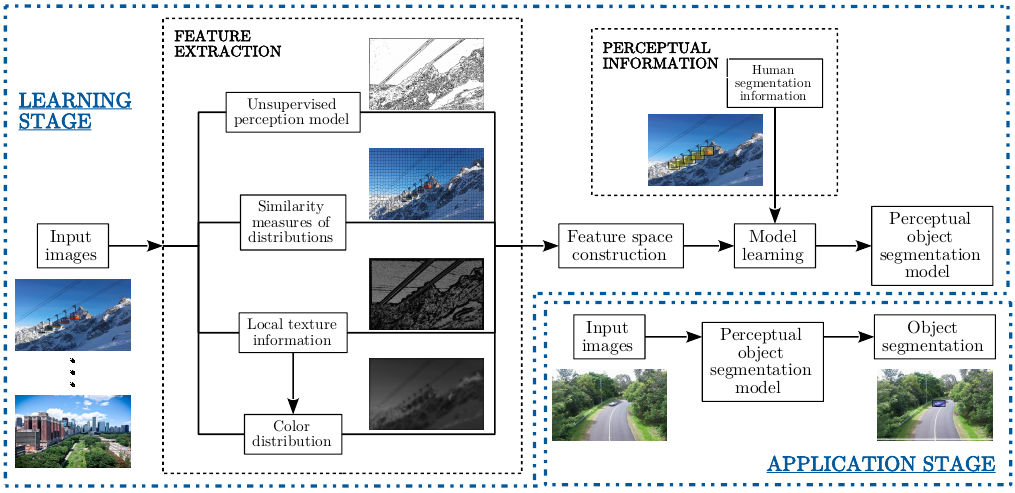
\includegraphics[width=\textwidth]{general_diagram}        
    \caption{(Draft) Proposed framework for object detection and scene understanding.}\label{fig:general_diagram_framework}
\end{figure}

Throughout the study of each of the low-level primitives and their resulting feautues, several secondary targets are present.

\begin{itemize}
	\item \textbf{Framework implementation.} Referring in a first stage to the implementation in simulated and off-board environments. In a second moment, to the implementation in a real platform. The latter requires the search for a portable platform capable of real-time operation.
 
	\item \textbf{Framework functional evaluation.} Comparison of the obtained results w.r.t. the approaches of state of the art.
 
 	\item \textbf{Framework validation.} Real test deployment taking into account the constraints of portability and real-time on the industrial scale.
 
\end{itemize}

Finally, this thesis aims to show that traditional computer vision methods are (still) a reliable option to develop the object detection and recognition. Especially in today's context, where there are hundreds of highly performing algorithms for image segmentation and object detection based on neural networks and artificial intelligence, however, these algorithms are in trouble when it comes to image analysis of complex scenarios or applications where there are no a database rich enough to do the learning process.


\section*{Organization of the Document}

We explore three low-level primitives during this thesis; contours, color and texture. The organization of this document follows to some extent the evolution of the construction of the vision-based framework to aid drone navigation. This thesis will then be decomposed into three parts:

\begin{enumerate}
	\item A part dedicated to the study of the contours of the image, in which we review in detail some of the classic methods for obtaining image contours. We use this information in conjunction with the \textit{a contrario} method and the Gestalt organizing laws to perform the detection and identification of landing targets.
	\item The second part is dedicated to the study of the color and texture of an image. In particular, we are interested in the global distribution of this information and the existing metrics to measure the similarity between the distributions. We apply and validate these concepts in a retrival image system.
	\item In the third and last part of this work, we extend the study of color and texture in images, this time we are interested in the local distribution of these primitives. We also study the influence of color information on the creation of textures in an image. We propose a completely unsupervised framework for the detection of perceptual bondaries. Furthermore, we explore different strategies to obtain the segmentation of natural images using the obtained perceptual boundaries.
\end{enumerate}

\begin{itemize}
	\item \textbf{Chapter}
	\item \textbf{Chapter}
	\item \textbf{Chapter}
	\item \textbf{Chapter}
	\item \textbf{Chapter}
	\item \textbf{Chapter}	
\end{itemize}